\documentclass[11pt,a4paper]{article}
\usepackage{TeX_definitions}
\geometry{left=2.4cm,right=2.4cm,top=2.4cm,bottom=2.4cm}
\graphicspath{{figures/}}
\hypersetup{colorlinks=true,linkcolor=blue,citecolor=blue,urlcolor=blue}

\title{Analysis 4-7: beyond map-colouring}
\author{}
\date{\today}
\begin{document}
\maketitle

\section{Question}
Analysis 4-7 asks how far the current programme can generalise beyond repulsive map-colouring. If the real scientific goal is to understand human structural approximation on graphs, then task domain matters.

\section{Method}
Standard graphical-model background and notation are treated in the usual way; see \cite{Koller2009}.


We compared map-colouring with four alternative graph-inference domains and scored each one on theoretical value, experimental simplicity, continuity with the current paradigm, and expected family discriminability. We also recorded how the Analysis 4 family taxonomy transfers to each domain.

\section{Results}
The highest-priority next domain is \texttt{attractive\_graph\_labelling}. Its main advantage is that it reverses local semantics from repulsive to attractive while preserving much of the current graph-based interface. The top three weighted-priority domains were \texttt{attractive\_graph\_labelling} (4.75), \texttt{map\_colouring} (4.1), and \texttt{social\_consensus} (4.0).

\begin{figure}[H]
\centering
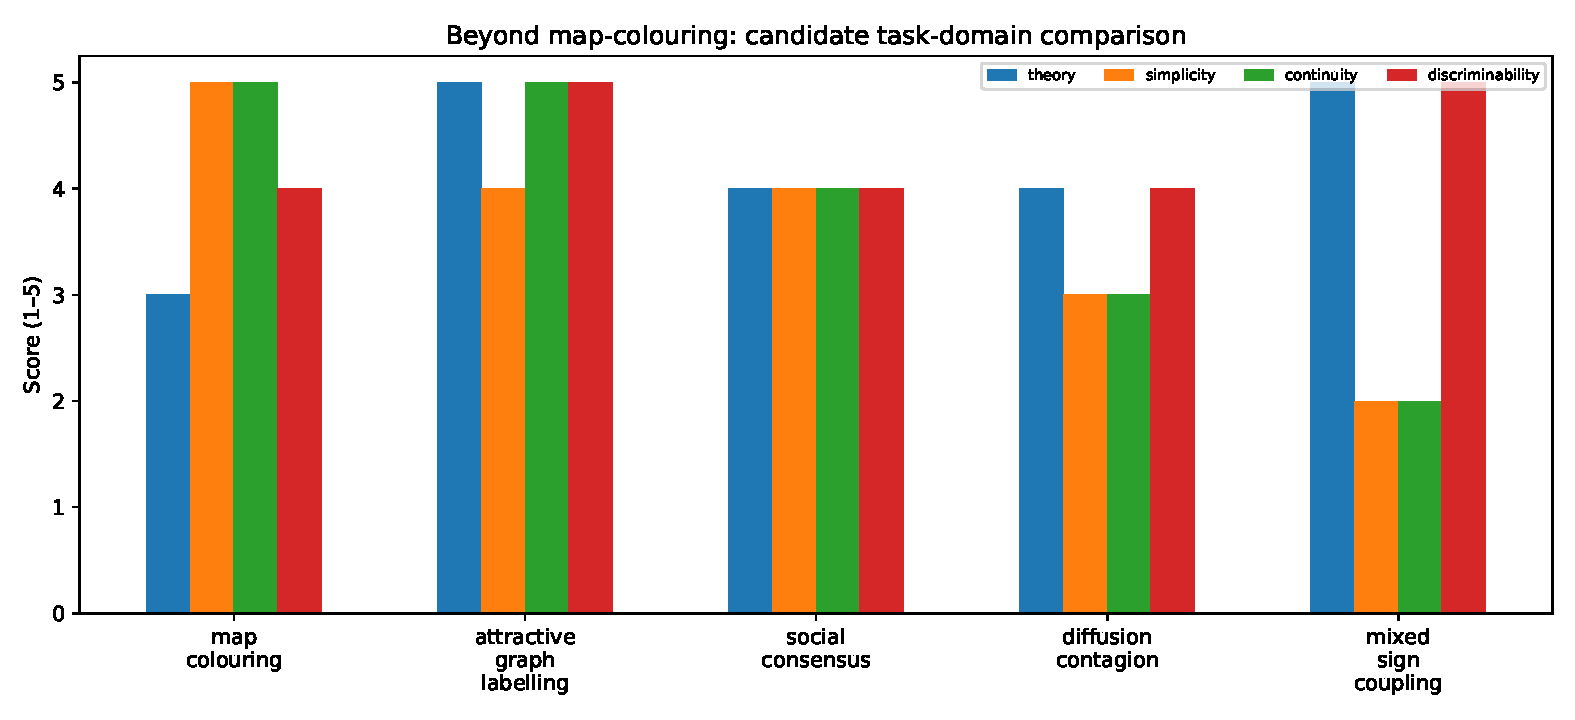
\includegraphics[width=\textwidth]{analysis-4-7_fig1_domain_comparison.pdf}
\caption{Comparison of candidate task domains beyond map-colouring.}
\end{figure}

\section{Conclusions against the TODO}
\begin{enumerate}
    \item Map-colouring remains a strong first testbed, but its claims should be limited to repulsive local couplings.
    \item Attractive graph labelling is the cleanest first extension.
    \item The current family taxonomy transfers well to attractive and consensus-style tasks, especially through $M_{\rho}$, $M_{\mathrm{star}}$, and $M_{\mathrm{cluster}}$.
    \item Mixed-sign tasks remain scientifically interesting but should be deferred until after a simpler attractive extension.
\end{enumerate}

\bibliographystyle{apalike}
\bibliography{../../manuscript/library}
\end{document}
